\documentclass{beamer}
\usetheme[white]{Wisconsin}
\usepackage{longtable}
\usepackage{listings}
\usepackage{color}
%% The amssymb package provides various useful mathematical symbols
\usepackage{amssymb}
%% The amsthm package provides extended theorem environments
\usepackage{amsthm} \usepackage{amsmath} \usepackage{tmadd,tmath}
\usepackage[mathcal]{euscript} \usepackage{color}
\usepackage{textcomp}
\usepackage{algorithm,algorithmic}
\definecolor{listinggray}{gray}{0.9}
\definecolor{lbcolor}{rgb}{0.9,0.9,0.9}
\lstset{
  backgroundcolor=\color{lbcolor},
  tabsize=4,
  rulecolor=,
  language=c++,
  basicstyle=\scriptsize,
  upquote=true,
  aboveskip={1.5\baselineskip},
  columns=fixed,
  showstringspaces=false,
  extendedchars=true,
  breaklines=true,
  prebreak =
  \raisebox{0ex}[0ex][0ex]{\ensuremath{\hookleftarrow}},
  frame=single,
  showtabs=false,
  showspaces=false,
  showstringspaces=false,
  identifierstyle=\ttfamily,
  keywordstyle=\color[rgb]{0,0,1},
  commentstyle=\color[rgb]{0.133,0.545,0.133},
  stringstyle=\color[rgb]{0.627,0.126,0.941},
}

%% colors
\setbeamercolor{boxheadcolor}{fg=white,bg=UWRed}
\setbeamercolor{boxbodycolor}{fg=black,bg=white}


%%---------------------------------------------------------------------------%%
\author{Stuart R. Slattery
  \\ Engineering Physics Department
  \\ University of Wisconsin - Madison
}

\date{\today} 
\title{Data Transfer Kit Summary}
\begin{document}
\maketitle

%%---------------------------------------------------------------------------%%
\begin{frame}{Outline}

  \begin{itemize}
  \item Overview
    \medskip
  \item Concepts and Geometric Rendezvous
    \medskip
  \item DTK Algorithms
    \medskip
  \item Code Example
  \end{itemize}

\end{frame}

%%---------------------------------------------------------------------------%%
\begin{frame}{What is DTK?}

  \begin{itemize}
  \item Collection of geometry-based data mapping algorithms for
    shared domain probelems
    \medskip
  \item Data maps allow for efficient movement of data in parallel
    (e.g. between meshes of a different parallel decomposition)
    \medskip
  \item Ideally maps are generated at a desireable time complexity
    (logarithmic)
    \medskip
  \item Input mesh and geometry data drive the map generation
    \medskip
  \item Should be viewed as a service providing suite of concrete
    algorithm implementations
  \end{itemize}
 
\end{frame}

%%---------------------------------------------------------------------------%%
\begin{frame}{What DTK Doesn't Do}

  \begin{itemize}
  \item Does not provide a general interface for all physics codes to
    couple to all other physics codes
    \medskip
  \item Does not provide discretization services (e.g. basis functions)
    \medskip
  \item Does not provide algorithm implementations for interface-based
    data transfer
    \medskip
  \item Does not allocate or deallocate memory in user code
  \end{itemize}

\end{frame}

%%---------------------------------------------------------------------------%%
\begin{frame}{Software Overview}

  \begin{itemize}
  \item Preliminary development of mesh-based capabilities during
    summer 2012 CASL internship at ORNL
    \medskip
  \item Additional development of geometry-based capabilities during
    fall 2012
    \medskip
  \item Implemented in C++
    \medskip
  \item Heavy use of the Trilinos scientific computing libraries
    \medskip
  \item Continuous and nightly testing as part of the CASL CDash
    system
    \medskip
  \item Open-source BSD 3-clause license
    \medskip
  \item https://github.com/CNERG/DataTransferKit
  \end{itemize}
  
\end{frame}

%%---------------------------------------------------------------------------%%
\begin{frame}{Concepts and Geometric Rendezvous}

\end{frame}

%%---------------------------------------------------------------------------%%
\begin{frame}{Communicators}

  \begin{columns}
    
    \begin{column}{0.5\textwidth}
      \begin{itemize}
      \item DTK handles source and target communicators of arbitrary
        relation 
        \medskip
      \item Any amount of overlap or lack thereof supported
        \medskip
      \item A global communicator required (doesn't have to be
        MPI\_COMM\_WORLD) 
      \end{itemize}
    \end{column}

    \begin{column}{0.5\textwidth}
      \begin{figure}[htpb!]
        \centering 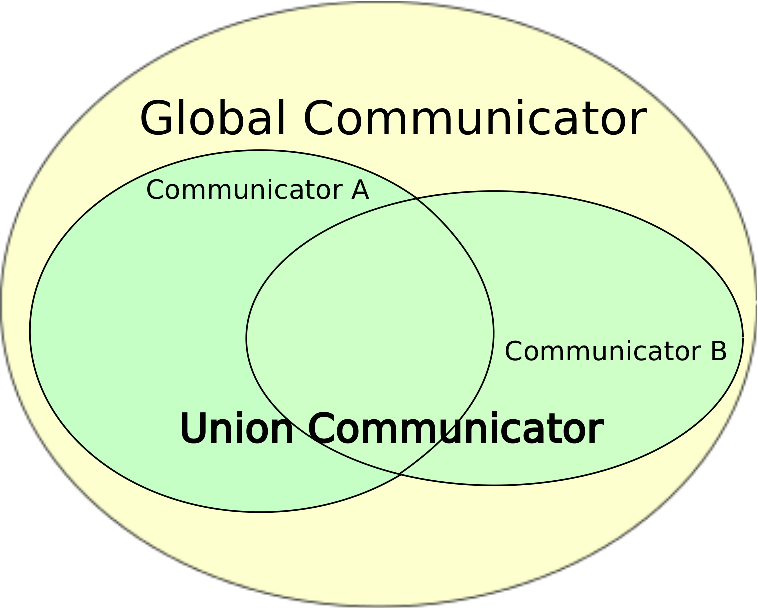
\includegraphics[width=1.7in]{union_comm.pdf}
      \end{figure}

      \begin{figure}[htpb!]
        \centering 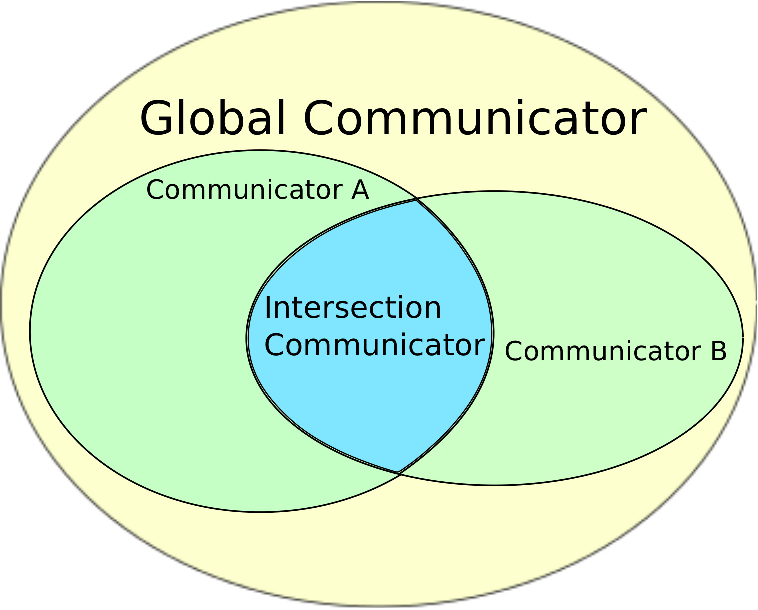
\includegraphics[width=1.7in]{intersection_comm.pdf}
      \end{figure}
    \end{column}

  \end{columns}

\end{frame}

%%---------------------------------------------------------------------------%%
\begin{frame}{Shared Domain Problems}

  \begin{columns}
    
    \begin{column}{0.5\textwidth}
      \begin{figure}[htpb!]
        \centering 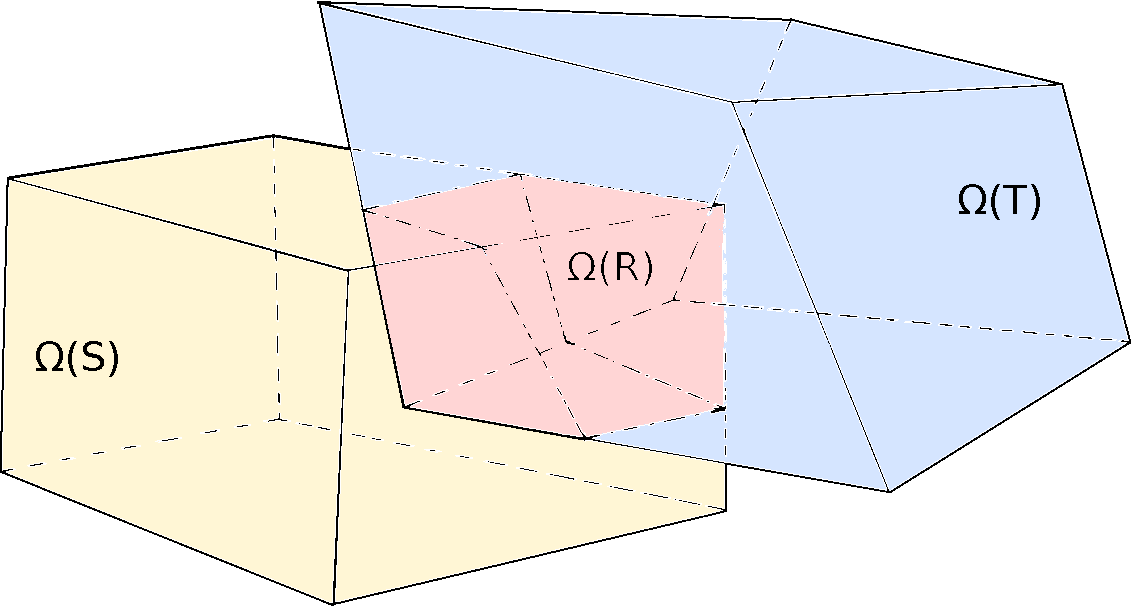
\includegraphics[width=2.5in]{overlapping_domain.pdf}
        \caption{\bf \sl Shared domain example.} {\sl $\Omega(S)$ (yellow)
          is the source geometry, $\Omega(T)$ (blue) is the target geometry,
          and $\Omega(R)$ (red) is the shared domain.}
        \label{fig:shared_domain}
      \end{figure}
    \end{column}

    \begin{column}{0.5\textwidth}
      \begin{itemize}
      \item Defined over a communicator that encapsulates the union of
        the source and target communicators
        \medskip
      \item Source and target must be of same geometric dimension
        \medskip
      \item The rendezvous algorithm leveraged to provide parallel
        topology maps for shared domains
      \end{itemize}
    \end{column}

  \end{columns}

\end{frame}

%%---------------------------------------------------------------------------%%
\begin{frame}{Parallel Topology Maps}

  \begin{itemize}
  \item An operator, $\ve{M}$, that defines the translation of a
    field, $\ve{F}(s)$, from a source spatial domain, $\Omega_S$, to a
    field, $\ve{G}(t$), in the target spatial domain $\Omega_T$, such
    that $\ve{G}(t)\leftarrow \ve{M}(\ve{F}(s))$ and $\ve{M}:
    \mathbb{R}^D \rightarrow \mathbb{R}^D, \forall r \in \Omega_R$,
    where $\Omega_R$ is the geometric rendezvous of the source and
    target.
    \medskip
  \item $\ve{M}$ is in general expensive to generate but cheap to
    apply
    \medskip
  \item For static $\ve{F}(s)$ and $\ve{G}(t)$, building $\ve{M}$ is a
    one-time, upfront cost
  \end{itemize}

\end{frame}

%%---------------------------------------------------------------------------%%
\begin{frame}{The Rendezvous Algorithm}

  \begin{itemize}
    \item Initially developed by the SIERRA team in the mid-2000's for
      parallel mesh-based data transfer \footnote{S. Plimpton,
        B. Hendrickson, and J. Stewart, “A parallel rendezvous
        algorithm for interpolation between multiple grids,” Journal
        of Parallel and Distributed Computing, vol. 64, pp. 266–276,
        2004}
      \medskip
    \item Creates a parallel topology map that can be used repeatedly
      for data transfer
    \item Map execution uses asynchronous strategy (posts and waits)
      with minimal messages
    \item Effectively $N*log(N)$ time complexity for parallel topology
      map generation
      \medskip
    \item Relies on the generation of a secondary decomposition of the
      source and target meshes with a geometric-based paritioning
      (RCB)
  \end{itemize}

\end{frame}

%%---------------------------------------------------------------------------%%
\begin{frame}{The Rendezvous Decomposition}

  \begin{columns}

    \begin{column}{0.33\textwidth}
      \begin{figure}[htpb!]
        \centering 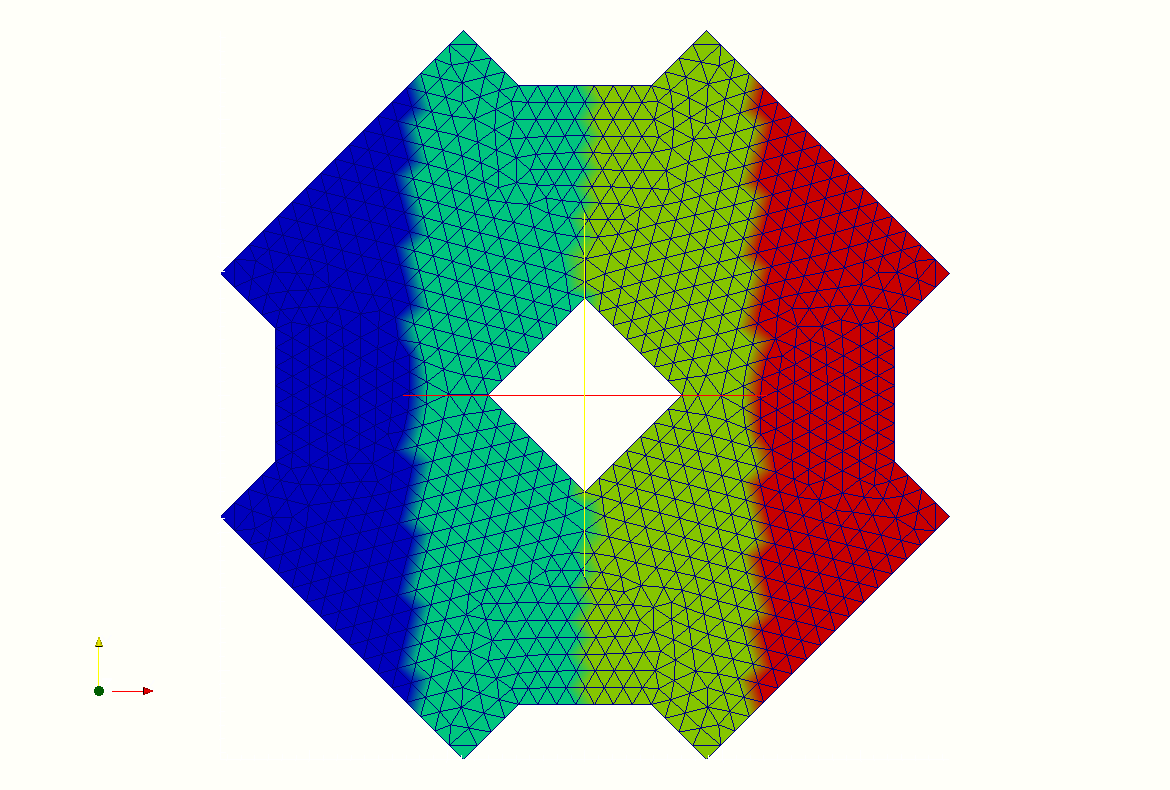
\includegraphics[width=2in]{tri_part.png}
        \caption{\small \sl Source mesh for 2D shared domain
          example.}
        \label{fig:source_mesh}
      \end{figure}
    \end{column}

    \begin{column}{0.33\textwidth}
      \begin{figure}[htpb!]
        \centering 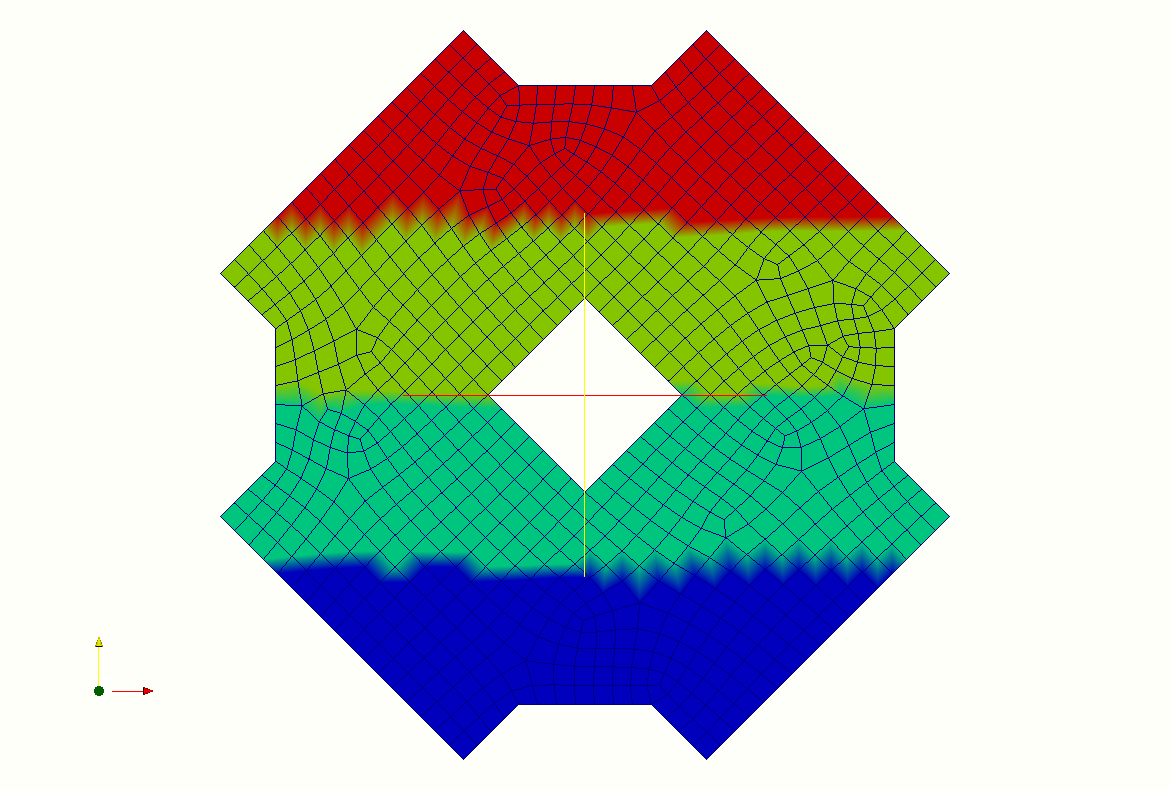
\includegraphics[width=2in]{quad_part.png}
        \caption{\small \sl Target mesh for 2D shared domain
          example.}
        \label{fig:target_mesh}
      \end{figure}
    \end{column}

    \begin{column}{0.33\textwidth}
      \begin{figure}[htpb!]
        \centering 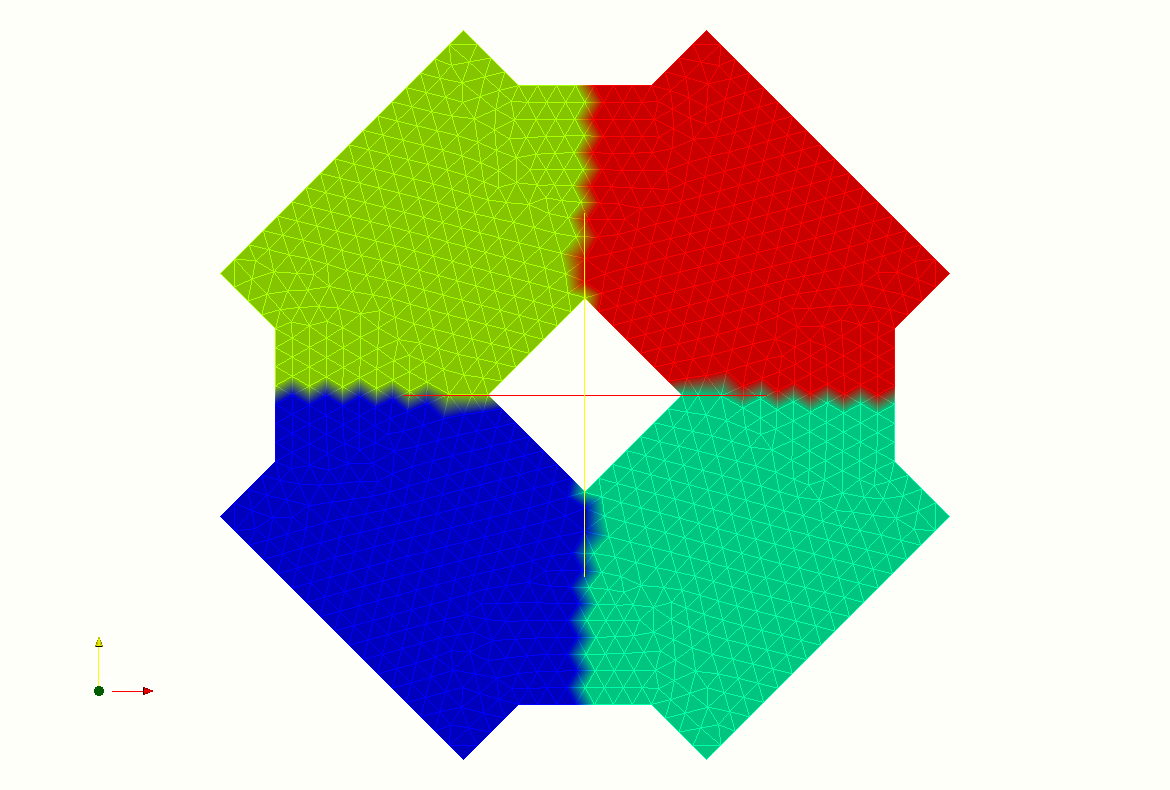
\includegraphics[width=2in]{tri_rend.png}
        \caption{\small \sl Rendezvous decomposition for 2D shared domain
          example.}
        \label{fig:rendezvous_part}
      \end{figure}
    \end{column}

  \end{columns}

\end{frame}

%%---------------------------------------------------------------------------%%
\begin{frame}{Searching the Rendezvous Decomposition}
  
  \begin{itemize}
  \item Hierarchical parallel search tree
    \medskip
  \item Rendezvous decomposition provides parallel search
    \medskip
  \item kD-tree provides on-process proximity search
    \medskip
  \item Newton iterations provide final point location
    \medskip
  \item Results in reasonable scalability
  \end{itemize}

\end{frame}

%%---------------------------------------------------------------------------%%
\begin{frame}{DTK Implementation Scaling Results}

  \begin{columns}
    
    \begin{column}{0.5\textwidth}
      \begin{itemize}
      \item Mesh-to-mesh transfer
      \item Worst case scenario study (all-to-all) with random points
        \medskip
      \item Qualitatively similar to the SIERRA results
        \medskip
      \item Largest test problems so far over 1.0E9 elements and 1.0E5
        cores
      \end{itemize}
    \end{column}

    \begin{column}{0.5\textwidth}
      \centering
      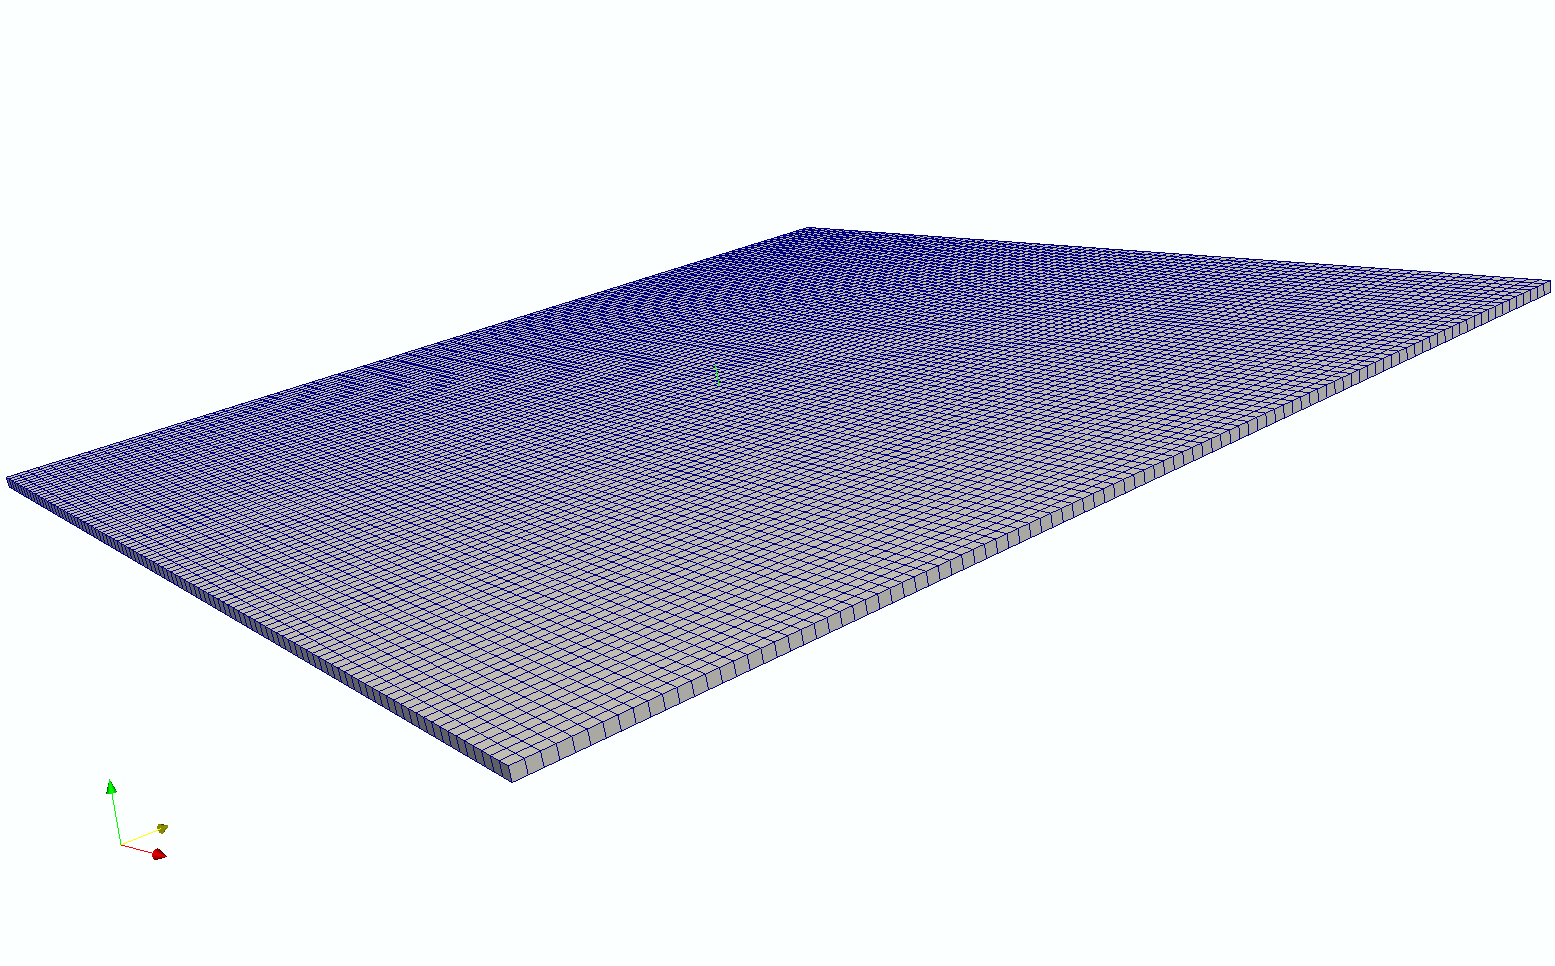
\includegraphics[width=2.4in]{mesh.png}
    \end{column}

  \end{columns}

\end{frame}

%%---------------------------------------------------------------------------%%
\begin{frame}{Strong Scaling}

  \begin{figure}[htpb!]
    \centering
    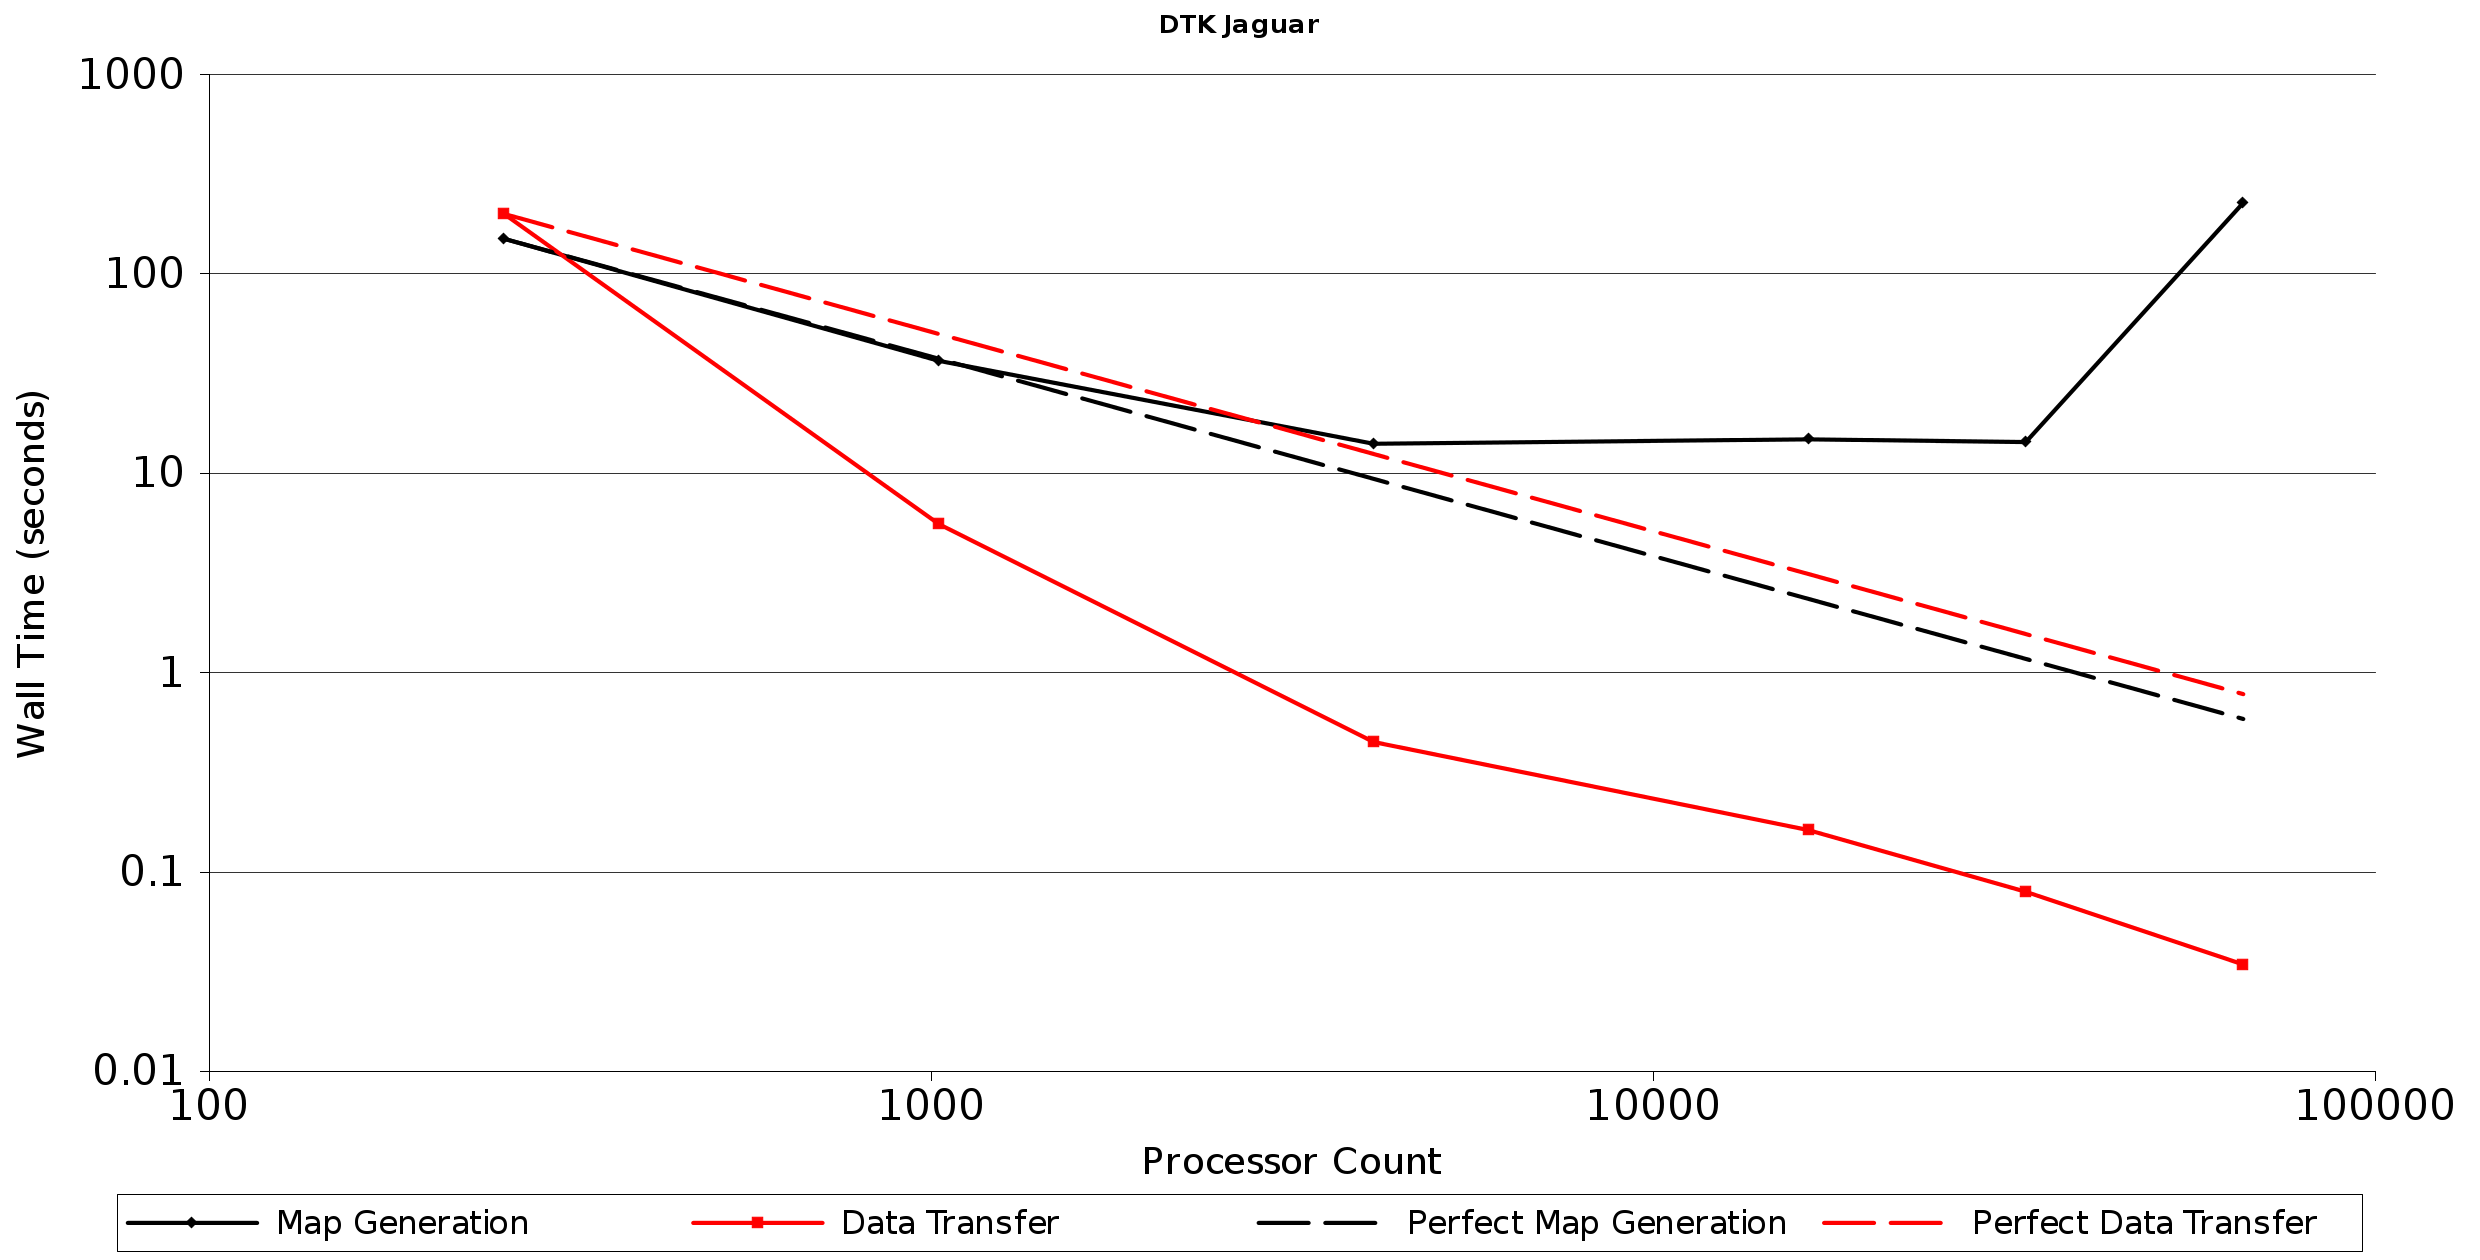
\includegraphics[width=4in]{StrongScaling.png}
    \caption{Strong scaling study results. The solid black curve reports
      the wall time to generate the mapping vs. number of processors
      while the solid red curve reports the wall time to transfer the
      data vs. number of processors. The dashed lines give
      perfect strong scaling the map generation (black) and the data
      transfer (red).}
    \label{fig:strong_scaling}
  \end{figure}

\end{frame}

%%---------------------------------------------------------------------------%%
\begin{frame}{Weak Scaling}

  \begin{figure}[ht!]
    \centering
    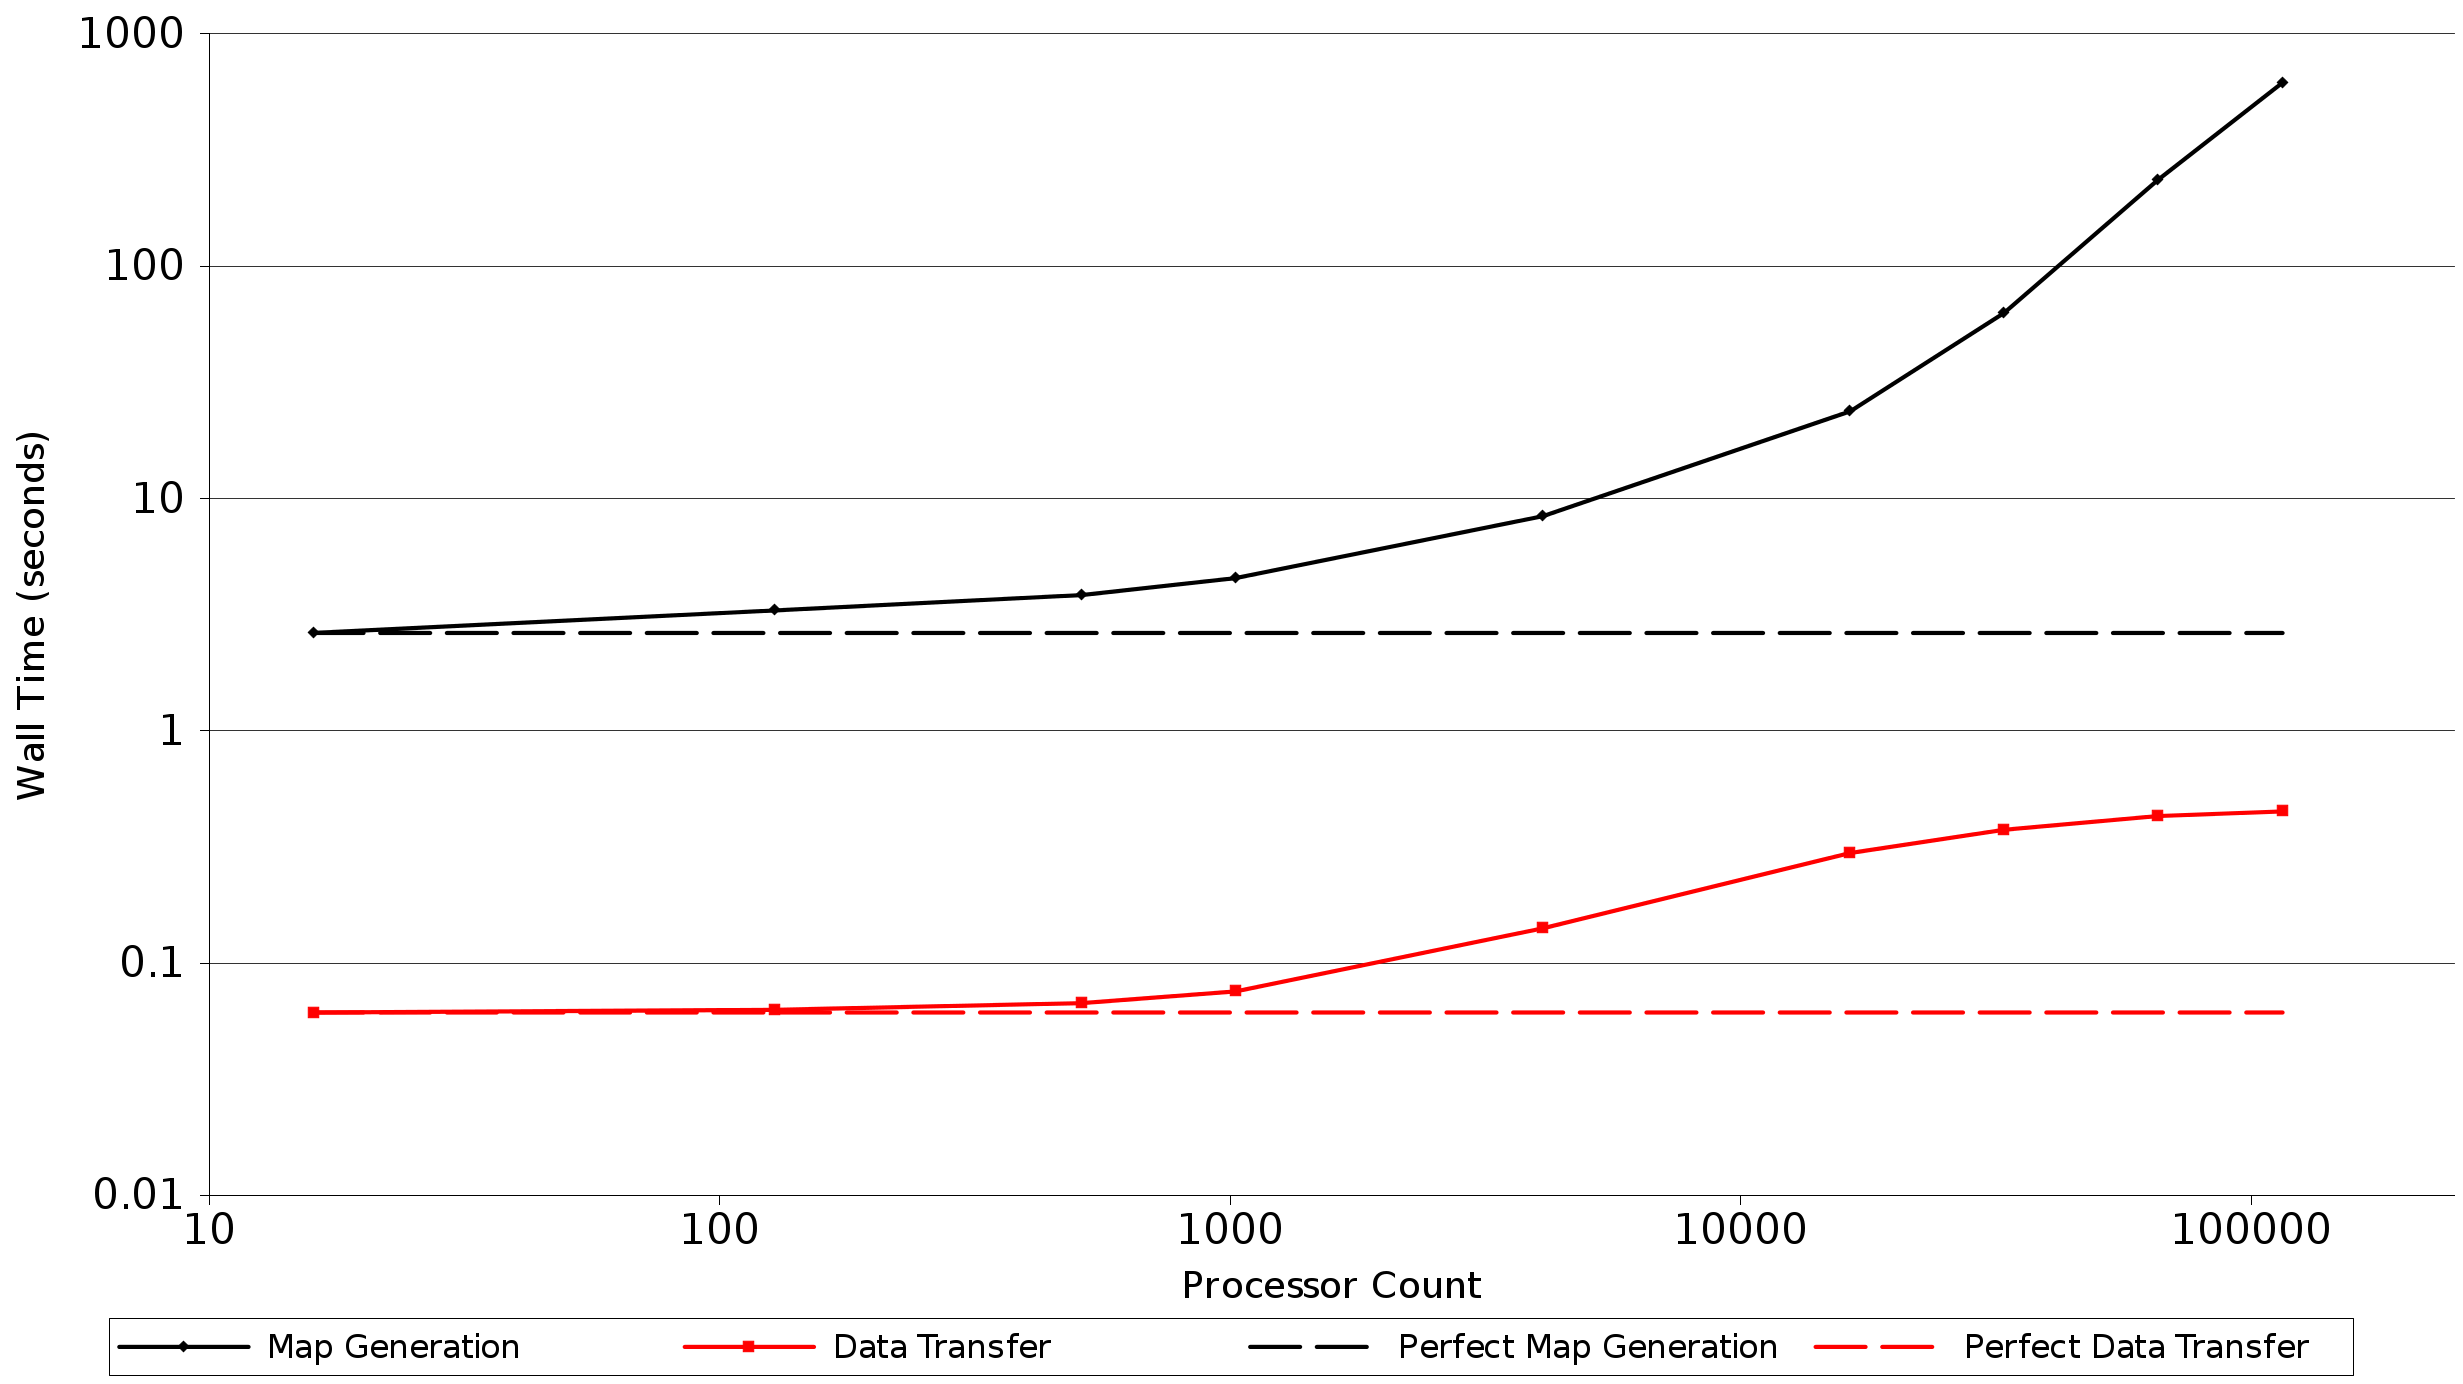
\includegraphics[width=4in]{WeakScaling.png}
    \caption{Weak scaling study results. The solid black curve reports
      the wall time to generate the mapping vs. number of processors
      while the solid red curve reports the wall time to transfer the
      data vs. number of processors. The dashed lines give
      perfect weak scaling the map generation (black) and the data
      transfer (red).}
    \label{fig:weak_scaling}
  \end{figure}

\end{frame}

%%---------------------------------------------------------------------------%%
\begin{frame}{Getting Data into DTK: Mesh}
  
  \begin{itemize}
    \item Meshes are viewed as geometric structures
      \medskip
    \item A subset of total mesh information is needed:
      \medskip
      \begin{itemize}
        \item Vertex coordinates
        \item Element topology
        \item Element connectivity
        \item Connectivity permutation
      \end{itemize}
      \medskip
    \item Parallel information is not required
      \medskip
    \item A communicator and global IDs are required
  \end{itemize}

\end{frame}

%%---------------------------------------------------------------------------%%
\begin{frame}{Mesh Vertices and Elements}

  \begin{columns}
    
    \begin{column}{0.5\textwidth}
      \begin{figure}[htpb!]
        \centering 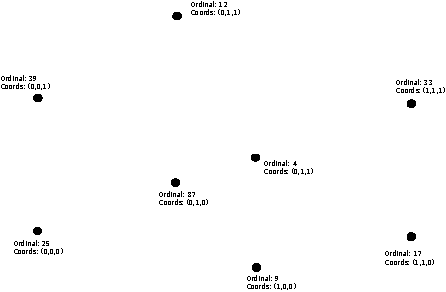
\includegraphics[width=2.25in]{hex_nodes.pdf}
        \caption{\bf \sl Basic vertex description for a mesh.}{\sl
          Each vertex is required to have a unique global ID}
      \end{figure}
    \end{column}

    \begin{column}{0.5\textwidth}
      \begin{figure}[htpb!]
        \centering 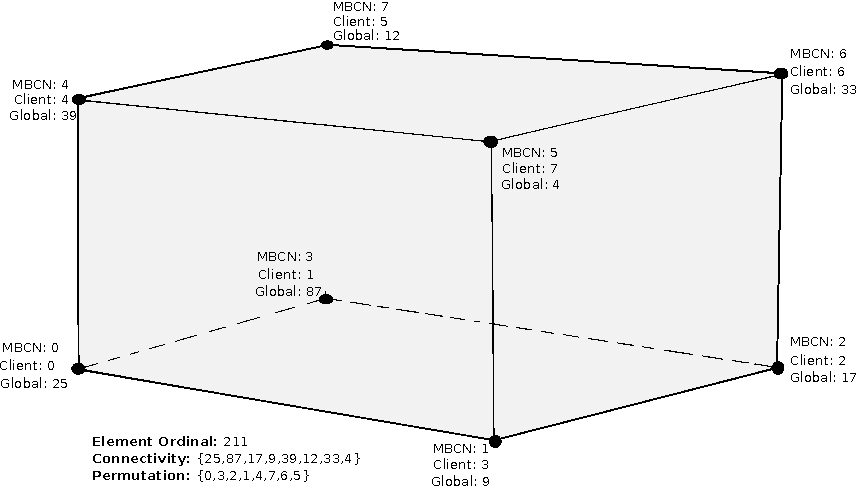
\includegraphics[width=2.25in]{hex_element.pdf}
        \caption{\bf \sl Basic element description for a mesh.}{\sl
          Each element is required to have a unique global ID}
      \end{figure}
    \end{column}

  \end{columns}

\end{frame}

%%---------------------------------------------------------------------------%%
\begin{frame}{Connectivity Permutation}

  \begin{columns}
    
    \begin{column}{0.5\textwidth}
      \begin{figure}[htpb!]
        \centering
        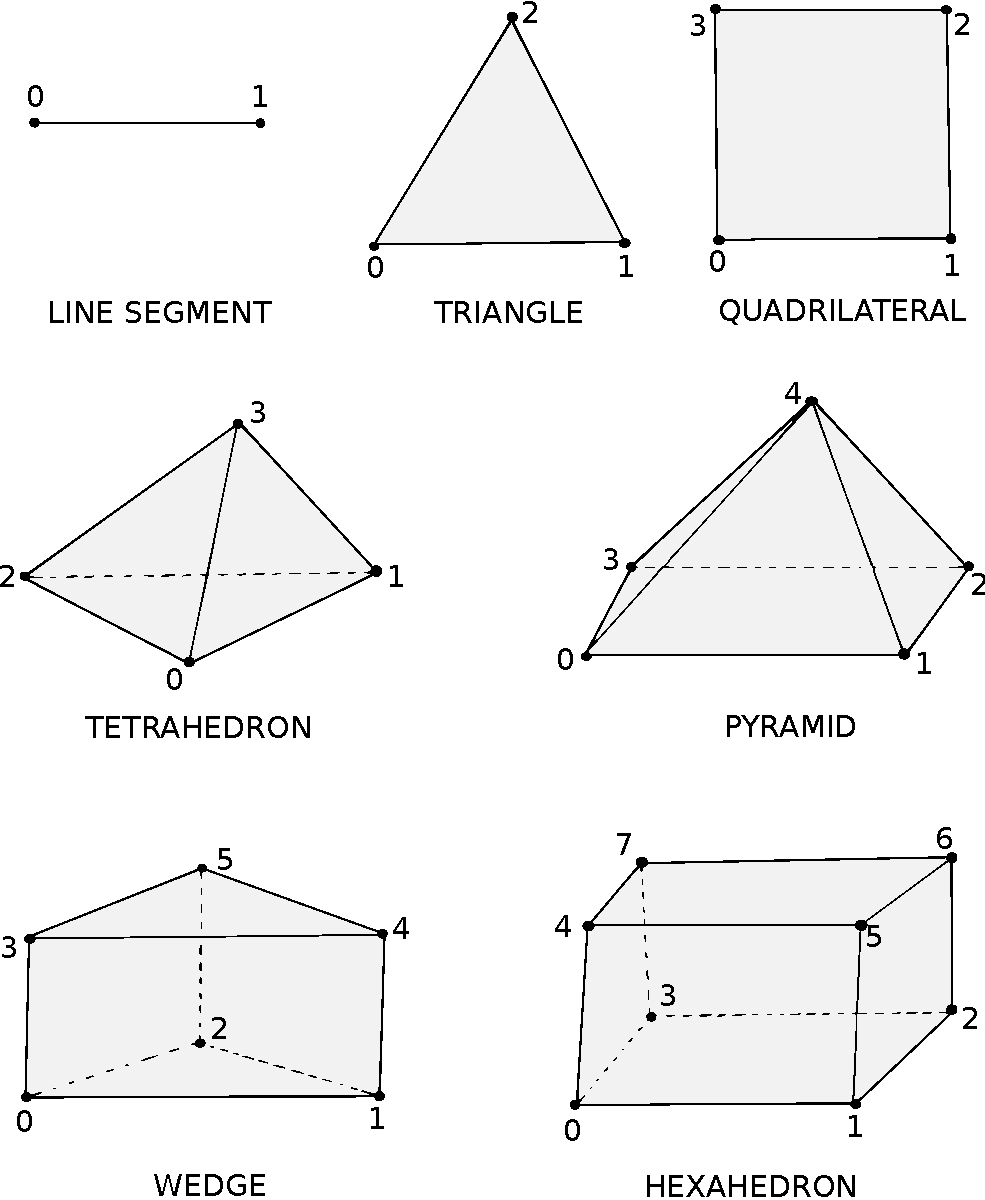
\includegraphics[width=2.2in]{Linear_Elements.pdf}
        \caption{\bf \sl Canonical vertex connectivity schemes for elements
          in DTK.}
        \label{fig:linear_elements}
      \end{figure}
    \end{column}

    \begin{column}{0.5\textwidth}
      \begin{itemize}
        \item Allow for user specification of canonical ordering
          \medskip
        \item Permutation list specifies the variation in ordering for
          a specified topology
          \medskip
        \item Other mesh topologies currently not supported
      \end{itemize}
    \end{column}

  \end{columns}


\end{frame}

%%---------------------------------------------------------------------------%%
\begin{frame}{Meshes of Multiple Topologies}

  \begin{itemize}
  \item All topologies in a mesh must be of the same dimension
  \item Each topology contained in a block
  \item Can have multiple blocks of the same topology
  \end{itemize}


  \begin{figure}[htpb!]
    \centering 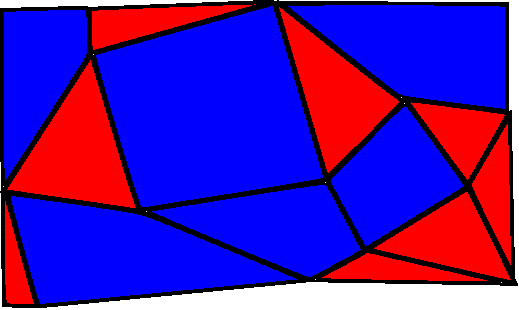
\includegraphics[width=2.5in]{hybrid_mesh.pdf}
    \caption{\bf \sl Hybrid mesh example.} {\sl Quadrilaterals (blue)
      must be specified in a different mesh block than the triangles
      (red). Both blocks can contain the mutual mesh vertices that
      construct their elements.}
    \label{fig:hybrid_mesh}
  \end{figure}

\end{frame}

%%---------------------------------------------------------------------------%%
\begin{frame}{Getting Data into DTK: Geometry}
  
  \begin{itemize}
  \item DTK's perception of general geometric structures is primitive
    \medskip
  \item A more capable geometry engine required for advanced
    algorithms
    \medskip
  \item A subset of total geometry information is needed:
    \medskip
    \begin{itemize}
    \item Centroid
    \item Bounding box
    \item Measure
    \item Point inclusion
    \end{itemize}
    \medskip
  \item Parallel information is not required
    \medskip
  \item A communicator and global IDs are required
  \end{itemize}

\end{frame}

%%---------------------------------------------------------------------------%%
\begin{frame}{Getting Data into DTK: Field Evaluations}

  \begin{itemize}
  \item Actual discretization of the field is not explicitly
    formulated
    \medskip
  \item Access to discretization of fields is generated through user
    code function evaluations at points in physical space:
    \medskip
  \end{itemize}

  \[
  \hat{f} \leftarrow \ve{F}(\hat{r}), \forall \hat{r} \in \Omega
  \]

  \begin{itemize}
  \item In the context of $\Omega$ discretized by a mesh, these
    evaluations can instead be written in terms of a single mesh
    element, $\omega \in \Omega$:
  \end{itemize}

  \[
  \hat{f} \leftarrow \ve{F}(\hat{r}), \forall \hat{r} \in \omega
  \]

\end{frame}

%%---------------------------------------------------------------------------%%
\begin{frame}{Getting Data into DTK: Field Evaluations}

  \begin{itemize}
    \item What user code should expect:
      \medskip
      \begin{itemize}
      \item A list of global element IDs that are on-process ($\omega$)
      \item A corresponding list of point coordinates ($\hat{r}$)
      \end{itemize}
      \medskip
    \item What user code should provide:
      \medskip
      \begin{itemize}
      \item A list of the resulting function evaluations for each
        global element ID/point coordinate pair provided ($\hat{f}$)
      \end{itemize}
    \item All data provided to user code will be local with respect to
      input data
    \item C++ inheritance (mix-in interface)
  \end{itemize}

\end{frame}

%%---------------------------------------------------------------------------%%
\begin{frame}{Getting Data into DTK: Field Integrations}

  \begin{itemize}
  \item Consider a measure-weighted integral:
  \end{itemize}

  \[
  f_{\Omega} = \frac{\int_{\Omega} \ve{F}(r) dr}{\int_{\Omega} dr}
  \]

  \begin{itemize}
  \item In the context of $\Omega$ discretized by a mesh, these
    evaluations can instead be written in terms of a single mesh
    element, $\omega \in \Omega$:
  \end{itemize}

  \[
  f_{\omega} = \int_{\omega} \ve{F}(r) dr
  \]

  \begin{itemize}
  \item The integral over $\Omega$ will be the measure-weighted
    summation of all element integrals:
  \end{itemize}

  \[
    f_{\Omega} = \frac{1}{m_{\Omega}} \sum_i f_{{\omega}_i},\ \forall
    \omega_i \in \Omega
  \]

  \begin{itemize}
  \item Element-wise spatial integrals generated through user code
  \end{itemize}
\end{frame}

%%---------------------------------------------------------------------------%%
\begin{frame}{Getting Data into DTK: Field Integrations}

  \begin{itemize}
    \item What user code should expect:
      \medskip
      \begin{itemize}
      \item A list of global element IDs that are on-process ($\omega$)
      \end{itemize}
      \medskip
    \item What user code should provide:
      \medskip
      \begin{itemize}
      \item A list of the resulting function integrations for each
        global element ID provided ($f_{\omega}$)
      \end{itemize}
    \item All data provided to user code will be local with respect to
      input data
    \item C++ inheritance (mix-in interface)
  \end{itemize}

\end{frame}

%%---------------------------------------------------------------------------%%
\begin{frame}{Getting Data into DTK: Target Data Space}

  \begin{itemize}
    \item What user code should provide:
      \medskip
      \begin{itemize}
      \item Allocated memory block large enough to hold the resulting
        function evaluations or integrations for the specified local
        target objects
      \end{itemize}
    \item What user code should expect:
      \medskip
      \begin{itemize}
      \item No allocation of memory
      \item A result of 0 if no evaluation or integration occurred for
        that object
      \end{itemize}
      \medskip
    \item All data provided to user code will be local with respect to
      input data
    \item Implemented as array views (pointer and size)
  \end{itemize}

\end{frame}

%%---------------------------------------------------------------------------%%
\begin{frame}{Standard Mesh-Based Rendezvous Map}

  \begin{columns}
    
    \begin{column}{0.5\textwidth}
      \begin{figure}
      \centering
      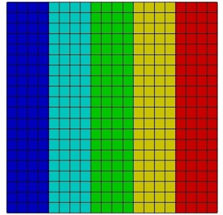
\includegraphics[width=1.25in]{neutronics_parallel_decomp.png}
      \end{figure}

      \begin{figure}
      \centering
      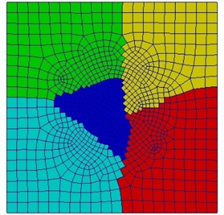
\includegraphics[width=1.25in]{cfd_parallel_decomp.png}
      \end{figure}
    \end{column}

    \begin{column}{0.5\textwidth}
      \begin{itemize}
      \item Mesh-to-Mesh transfer \footnote{Example provided by Roger
        Pawlowski}
        \medskip
      \item Used to move $\ve{F}(\hat{r})$ between meshes of arbitrary
        distribution
        \medskip
      \item Requires user code for evaluations in mesh elements
      \end{itemize}

      \begin{figure}
      \centering
      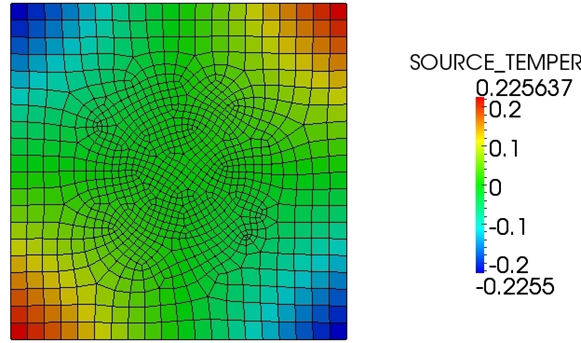
\includegraphics[width=1.75in]{cfd_transferred_field.png}
      \end{figure}
    \end{column}

  \end{columns}

\end{frame}

%%---------------------------------------------------------------------------%%
\begin{frame}{Other Rendezvous-Based Maps: Integral Assembly}

  \begin{columns}
    
    \begin{column}{0.4\textwidth}
      \begin{itemize}
      \item Mesh-to-geometry transfer
        \medskip
      \item Used to assemble $f_{\Omega}$ with mesh and geometry of
        arbitrary distribution into measure-weighted integral
        \medskip
      \item The mesh is assumed conformal
        \medskip
      \item Requires user code for integrations in mesh elements
        \medskip
      \item See example/IntegralAssembly
      \end{itemize}
    \end{column}

    \begin{column}{0.6\textwidth}
      \begin{figure}
      \centering
      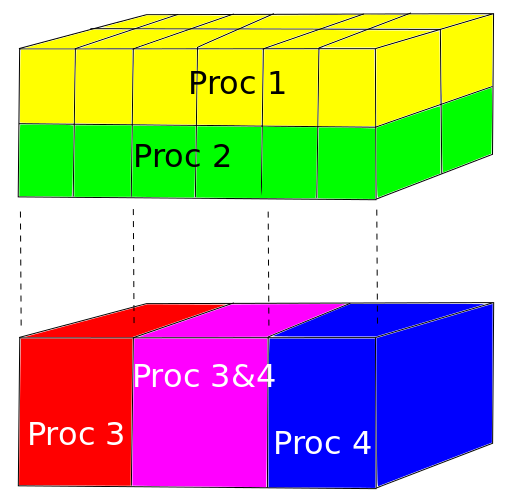
\includegraphics[width=2.5in]{integral_assembly.png}
      \end{figure}
    \end{column}

  \end{columns}

\end{frame}

%%---------------------------------------------------------------------------%%
\begin{frame}{Other Rendezvous-Based Maps: Geometry to Geometry}

  \begin{figure}
    \centering
    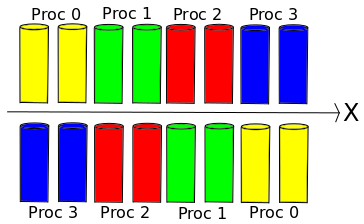
\includegraphics[width=2in]{volumetovolume.png}
  \end{figure}

  \begin{itemize}
  \item Simple geometry-to-geometry transfer capability
    \medskip
  \item Geometries are assumed conformal
    \medskip
  \item Requires user code for evaluations in geometry
    \medskip
  \item See example/GeometryToGeometry
  \end{itemize}

\end{frame}

%%---------------------------------------------------------------------------%%
\begin{frame}{Other Rendezvous-Based Maps: Geometry to Mesh}

  \begin{figure}
    \centering
    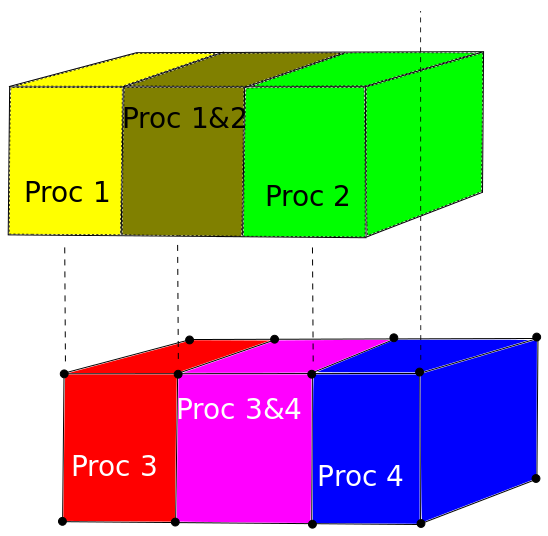
\includegraphics[width=2in]{volumetomesh.png}
  \end{figure}

  \begin{itemize}
  \item Similar to mesh-based rendezvous
    \medskip
  \item Does not require a mesh, conceptual in this case
    \medskip
  \item Requires user code for evaluations in geometry
    \medskip
  \item See example/GeometryToMesh
  \end{itemize}

\end{frame}

%%---------------------------------------------------------------------------%%
\begin{frame}{Super Simple Example}

  \begin{itemize}
  \item examples/WaveDamper
    \medskip
  \item Using DTK in the context of Picard iteration
    \medskip
  \item Start with existing codes, expose data to DTK
  \item Use mesh-to-mesh mapping in 1D
  \end{itemize}

  \begin{figure}
    \centering
    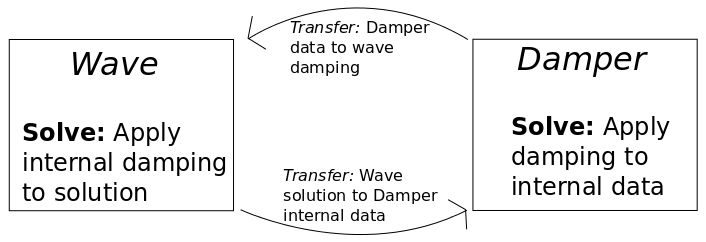
\includegraphics[width=4.5in]{wavedamperexample.png}
  \end{figure}

\end{frame}

%%---------------------------------------------------------------------------%%
\begin{frame}[fragile]{Super Simple Example: Wave}

  \begin{itemize}
  \item 1D code
  \item Initial conditions: $\ve{F}(x) = \cos(x)$
  \end{itemize}

  \begin{lstlisting}
    class Wave {
      private:
      Teuchos::RCP<const Teuchos::Comm<int> > comm;
      Teuchos::RCP<std::vector<double> > grid;
      Teuchos::RCP<std::vector<double> > data;
      Teuchos::RCP<std::vector<double> > damping;

      public:
      Wave( Teuchos::RCP<const Teuchos::Comm<int> > _comm,
      double x_min, double x_max, int num_x)
      {
        // Create the grid.
        // Set initial conditions.
      }

      void solve()
      { /* Apply the damping to the local data */ }
    };
  \end{lstlisting}

\end{frame}

%%---------------------------------------------------------------------------%%
\begin{frame}[fragile]{Super Simple Example: Damper}

  \begin{itemize}
  \item 1D code
  \item Initial conditions: none
  \end{itemize}

  \begin{lstlisting}
    class Damper
    {
      private:
      Teuchos::RCP<const Teuchos::Comm<int> > comm;
      Teuchos::RCP<std::vector<double> > data;
      Teuchos::RCP<std::vector<double> > damping;
      Teuchos::RCP<std::vector<double> > grid;

      public:
      Damper( Teuchos::RCP<const Teuchos::Comm<int> > _comm,
      double x_min, double x_max, int num_x)
      { /* Create the grid. */ }

      void solve()
      { /* Apply damping to the local data. */ }
    };
  \end{lstlisting}

\end{frame}

%%---------------------------------------------------------------------------%%
\begin{frame}[fragile]{Super Simple Example: Exposing Wave Data}

  \begin{itemize}
  \item Functions added to the Wave class
  \end{itemize}

  \begin{lstlisting}
    // Get the communicator.
    Teuchos::RCP<const Teuchos::Comm<int> > get_comm() const
    { return comm; }

    // Get a const reference to the local grid.
    const Teuchos::RCP<std::vector<double> >& get_grid() const
    { return grid; }

    // Get a reference to the local data.
    const Teuchos::RCP<std::vector<double> >& get_data() const
    { return data; }

    // Get a reference to the local data space storing 
    // the damping coefficients.
    Teuchos::RCP<std::vector<double> >& get_damping()
    { return damping; }
  \end{lstlisting}

\end{frame}

%%---------------------------------------------------------------------------%%
\begin{frame}[fragile]{Super Simple Example: Exposing Damper Data}

  \begin{itemize}
  \item Functions added to the Damper class
  \end{itemize}

  \begin{lstlisting}
    // Get the communicator.
    Teuchos::RCP<const Teuchos::Comm<int> > get_comm() const
    { return comm; }

    // Get a reference to the local damping data.
    Teuchos::RCP<std::vector<double> > get_damping() const
    { return damping; }

    // Get a reference to the local grid.
    Teuchos::RCP<std::vector<double> > get_grid() const
    { return grid; }

    // Get a reference to the memory space for external data 
    // to be applied to.
    Teuchos::RCP<std::vector<double> > get_external_data()
    { return data; }
  \end{lstlisting}

\end{frame}

%%---------------------------------------------------------------------------%%
\begin{frame}[fragile]{Super Simple Example: Wave Function Evaluations}

  \begin{itemize}
  \item Inherit from DataTransferKit::FieldEvaluator
  \item Implement the Evaluate() function
  \end{itemize}
 
  \begin{lstlisting}
  class WaveEvaluator : 
  public DataTransferKit::FieldEvaluator<ordinal_type,field_type>
  {
    public:
    WaveEvaluator( const RCP_Wave& wave );

    field_type evaluate( const Teuchos::ArrayRCP<int>& elements,
    const Teuchos::ArrayRCP<double>& coords )
    {
      // Setup an output field.
      // Get the Wave grid.
      // Get the Wave data.

      // Interpolate the Wave data onto the given 
      // coordinates using a linear basis. The 
      // coordinates will be valid for the given elements.
    }
  };
  \end{lstlisting}

\end{frame}

%%---------------------------------------------------------------------------%%
\begin{frame}[fragile]{Super Simple Example: Damper Function Evaluations}

  \begin{itemize}
  \item Inherit from DataTransferKit::FieldEvaluator
  \item Implement the Evaluate() function
  \end{itemize}
 
  \begin{lstlisting}
  class DamperEvaluator : 
  public DataTransferKit::FieldEvaluator<ordinal_type,field_type>
  {
    public:
    DamperEvaluator( const RCP_Damper& damper );

    field_type evaluate( const Teuchos::ArrayRCP<int>& elements,
    const Teuchos::ArrayRCP<double>& coords )
    {
      // Setup an output field.
      // Get the Damper grid.
      // Get the Damper data.

      // Interpolate the Damper data onto the given 
      // coordinates using a linear basis. The 
      // coordinates will be valid for the given elements.
    }
  };
  \end{lstlisting}

\end{frame}

%%---------------------------------------------------------------------------%%
\begin{frame}[fragile]{Super Simple Example: Wave Data Adapter}

  \begin{itemize}
  \item Provide DTK mesh and field data
  \end{itemize}
  
  \begin{lstlisting}
    class WaveAdapter
    {
      // Get the wave mesh.
      static RCP<DataTransferKit::MeshManager<MeshType> >
      getMesh( const RCP_Wave& wave );

      // Get the wave field evaluator.
      static RCP_Evaluator 
      getFieldEvaluator( const RCP_Wave& wave );

      // Get the wave target coordinates from the mesh.
      static RCP<DataTransferKit::FieldManager<MeshType> >
      getTargetCoords( const RCP_Wave& wave );

      // Get the wave target space.
      static RCP<DataTransferKit::FieldManager<FieldType> >
      getTargetSpace( const RCP_Wave& wave );
    };
  \end{lstlisting}

\end{frame}

%%---------------------------------------------------------------------------%%
\begin{frame}[fragile]{Super Simple Example: Damper Data Adapter}

  \begin{itemize}
  \item Provide DTK mesh and field data
  \end{itemize}
  
  \begin{lstlisting}
    class DamperAdapter
    {
      // Get the damper mesh.
      static RCP<DataTransferKit::MeshManager<MeshType> >
      getMesh( const RCP_Damper& damper );

      // Get the damper field evaluator.
      static RCP_Evaluator 
      getFieldEvaluator( const RCP_Damper& damper );

      // Get the damper target coordinates from the mesh.
      static RCP<DataTransferKit::FieldManager<MeshType> >
      getTargetCoords( const RCP_Damper& damper );

      // Get the damper target space.
      static RCP<DataTransferKit::FieldManager<FieldType> >
      getTargetSpace( const RCP_Damper& damper );
    };
  \end{lstlisting}

\end{frame}

%%---------------------------------------------------------------------------%%
\begin{frame}[fragile]{Super Simple Example: Driver Setup}

  \begin{lstlisting}
    int main(int argc, char* argv[])
    {
      // Parallel setup.
      Teuchos::RCP<const Teuchos::Comm<int> > comm_union;
      DataTransferKit::CommTools::unite( 
                          wave_comm, damper_comm, comm_union );
      // Wave setup.
      // Damper setup.
      // Mapping.
      DataTransferKit::SharedDomainMap<WaveAdapter::MeshType,
                                       DamperAdapter::MeshType>
          wave_to_damper_map( comm_union, 1 );
      wave_to_damper_map.setup(wave_mesh, damper_target_coords);

      DataTransferKit::SharedDomainMap<DamperAdapter::MeshType,
                                       WaveAdapter::MeshType>
          damper_to_wave_map( comm_union, 1 );
      damper_to_wave_map.setup(damper_mesh, wave_target_coords);

      // Solve. (next slide)
    }
  \end{lstlisting}

\end{frame}

%%---------------------------------------------------------------------------%%
\begin{frame}[fragile]{Super Simple Example: Driver Solve}

  \begin{itemize}
  \item Picard iterations to convergence
  \end{itemize}

  \begin{lstlisting}
    while( norm > tolerance && num_iter < max_iter )
    {
      wave_to_damper_map.apply( wave_evaluator, 
                                damper_target_space );

      damper->solve();

      damper_to_wave_map.apply( damper_evaluator, 
                                wave_target_space );

      wave->solve();
      
      // Compute Wave data norm.
      // Update the iteration count.
      // Barrier before proceeding to the next iteration.
    }
  \end{lstlisting}

\end{frame}

%%---------------------------------------------------------------------------%%

\end{document}
